\subsection{Standard Gradient Descent}

Für diese Variante gilt die Beziehung $ \vect{w_{neu}} = \vect{w} - \eta grad(f) $. Der geschriebene \textsc{Matlab}-Code befindet sich im Anhang.

Die folgenden Abbildungen stellen die Entwicklung des Gewichtsvektors $\vect{w}$ dar:

\begin{itemize}
  \item Abbildung~\ref{fig:path_w01_eta02} zeigt den Verlauf von $\vect{w}$ für $\vect{w_0} = \begin{bmatrix} 2 \\ 0.5 \end{bmatrix}$ und $\eta = 0.2$
  \item Abbildung~\ref{fig:path_w01_eta015} zeigt den Verlauf von $\vect{w}$ für $\vect{w_0} = \begin{bmatrix} 2 \\ 0.5 \end{bmatrix}$ und $\eta = 0.15$
  \item Abbildung~\ref{fig:path_w01_eta01} zeigt den Verlauf von $\vect{w}$ für $\vect{w_0} = \begin{bmatrix} 2 \\ 0.5 \end{bmatrix}$ und $\eta = 0.1$
  \item Abbildung~\ref{fig:path_w01_eta005} zeigt den Verlauf von $\vect{w}$ für $\vect{w_0} = \begin{bmatrix} 2 \\ 0.5 \end{bmatrix}$ und $\eta = 0.05$
  \item Abbildung~\ref{fig:error_w01} zeigt den Verlauf von $f(\vect{w})$ mit $\vect{w_0} = \begin{bmatrix} 2 \\ 0.5 \end{bmatrix}$ für alle $\eta = \{0.2, 0.15, 0.1, 0.05\}$
  \item Abbildung~\ref{fig:path_w02_eta02} zeigt den Verlauf von $\vect{w}$ für $\vect{w_0} = \begin{bmatrix} -0.2 \\ -0.5 \end{bmatrix}$ und $\eta = 0.2$
  \item Abbildung~\ref{fig:path_w02_eta015} zeigt den Verlauf von $\vect{w}$ für $\vect{w_0} = \begin{bmatrix} -0.2 \\ -0.5 \end{bmatrix}$ und $\eta = 0.15$
  \item Abbildung~\ref{fig:path_w02_eta01} zeigt den Verlauf von $\vect{w}$ für $\vect{w_0} = \begin{bmatrix} -0.2 \\ -0.5 \end{bmatrix}$ und $\eta = 0.1$
  \item Abbildung~\ref{fig:path_w02_eta005} zeigt den Verlauf von $\vect{w}$ für $\vect{w_0} = \begin{bmatrix} -0.2 \\ -0.5 \end{bmatrix}$ und $\eta = 0.05$
  \item Abbildung~\ref{fig:error_w02} zeigt den Verlauf von $f(\vect{w})$ mit $\vect{w_0} = \begin{bmatrix} -0.2 \\ -0.5 \end{bmatrix}$ für alle $\eta = \{0.2, 0.15, 0.1, 0.05\}$
\end{itemize}

Man erkennt, dass die Entwicklung der Gewichte stark von den Anfangswerten und der Lernrate abhängt. Die ersten 4 Abbildungen (Abb.~\ref{fig:path_w01_eta02} bis Abb.~\ref{fig:path_w01_eta005}) zeigen den Verlauf für ein Anfangsgewicht, welches dem kleineren Minimum nahe liegt. Ist jedoch die Lernrate zu hoch ($\eta = \{0.2, 0.15\}$), bewegt sich der Verlauf ``zu schnell'' durch die Funktion, überspringt das kleine globale Minimum und landet im großen lokalen Minimum. Bei einer richtigen Lernrate ($\eta = 0.1$) landet der Verlauf im globalen Minimum und bleibt auch dort. Wählt man die Lernrate zu klein ($\eta = 0.05$), so ``verhungert'' der Verlauf und erreicht keines der Minima. Dieses Verhalten ist auch im Verlauf von $f(\vect{w})$ zu erkennen (Abb.~\ref{fig:error_w01}).

Bei einer anderen Wahl der Startgewichte (Abbildungen \ref{fig:path_w02_eta02} bis \ref{fig:path_w02_eta005}) erreicht der Verlauf nie das globale Minimum, da das lokale ``näher'' liegt. Im Verlauf von $f(\vect{w})$ (Abb.~\ref{fig:error_w02}) erkennt man, dass sich der Fehler umso schneller dem Minimum annähert, je größer die Lernrate ist.

Kurz gesagt: ist die Lernrate zu hoch, erreicht man zwar schnell ein Minimum, es besteht jedoch die Gefahr, dass ein Minimum, dass sich nur in einem kleinen, begrenzten Bereich befindet, übersprungen wird. Ist die Lernrate jedoch zu gering, kann die Anzahl der Iterationsschritte zu wenig sein, um überhaupt ein Minimum zu erreichen.


\begin{figure}[h!]
  \centering
  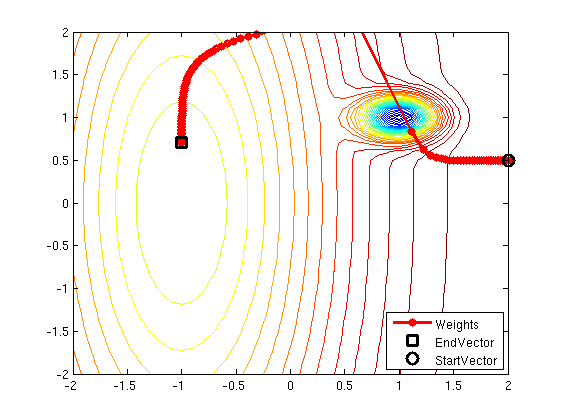
\includegraphics[width=0.8\textwidth]{./figures/211/path_w01_eta02.png}
  \caption{Verlauf von $\vect{w}$}
  \label{fig:path_w01_eta02}
\end{figure}

\begin{figure}[h!]
  \centering
  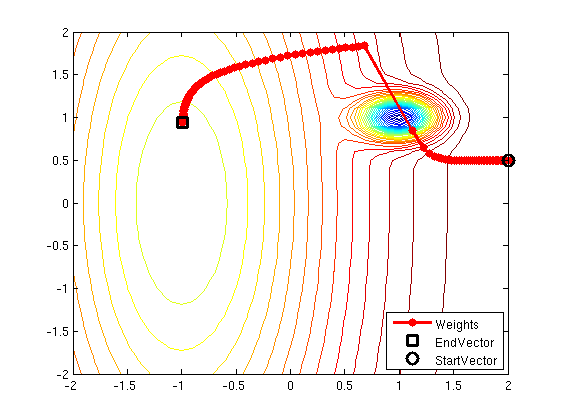
\includegraphics[width=0.8\textwidth]{./figures/211/path_w01_eta015.png}
  \caption{Verlauf von $\vect{w}$}
  \label{fig:path_w01_eta015}
\end{figure}

\begin{figure}[h!]
  \centering
  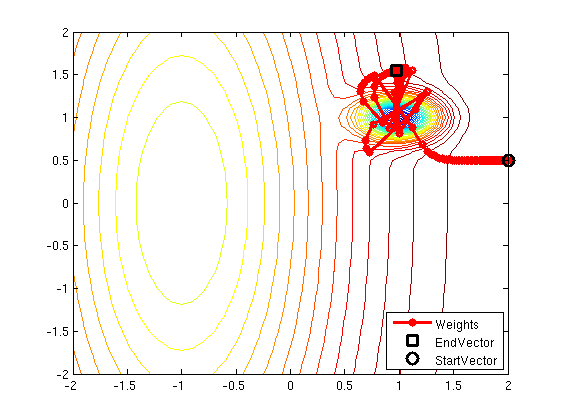
\includegraphics[width=0.8\textwidth]{./figures/211/path_w01_eta01.png}
  \caption{Verlauf von $\vect{w}$}
  \label{fig:path_w01_eta01}
\end{figure}

\begin{figure}[h!]
  \centering
  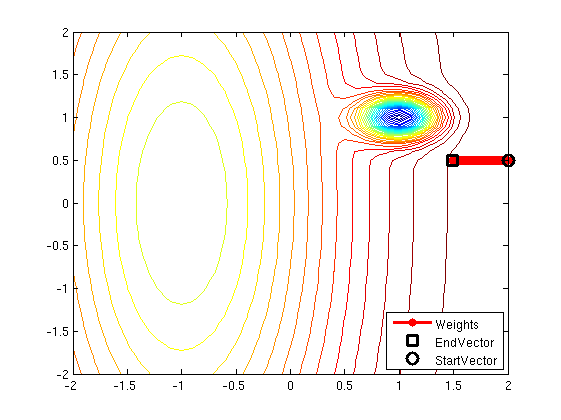
\includegraphics[width=0.8\textwidth]{./figures/211/path_w01_eta005.png}
  \caption{Verlauf von $\vect{w}$}
  \label{fig:path_w01_eta005}
\end{figure}

\begin{figure}[h!]
  \centering
  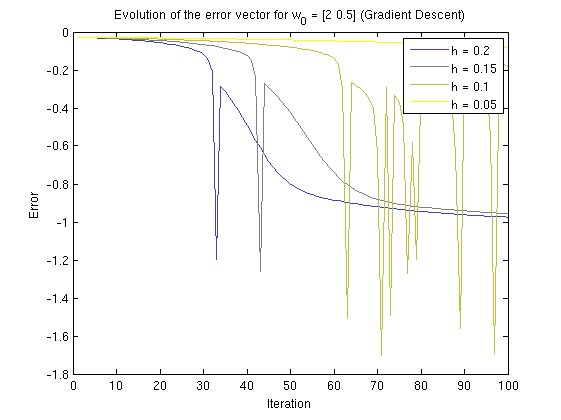
\includegraphics[width=0.8\textwidth]{./figures/211/error_w01.png}
  \caption{Verlauf von $f(\vect{w})$}
  \label{fig:error_w01}
\end{figure}

\begin{figure}[h!]
  \centering
  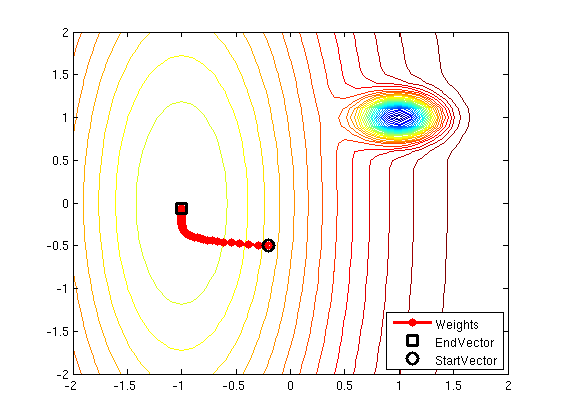
\includegraphics[width=0.8\textwidth]{./figures/211/path_w02_eta02.png}
  \caption{Verlauf von $\vect{w}$}
  \label{fig:path_w02_eta02}
\end{figure}

\begin{figure}[h!]
  \centering
  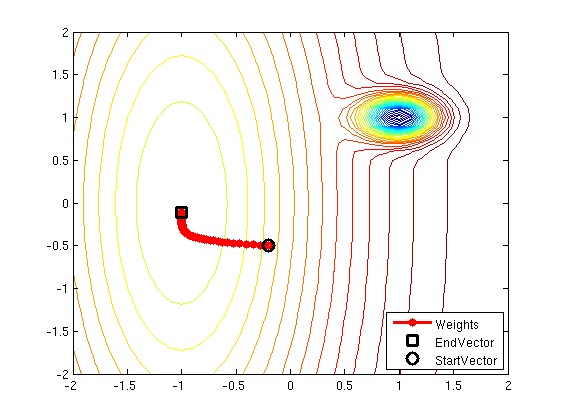
\includegraphics[width=0.8\textwidth]{./figures/211/path_w02_eta015.png}
  \caption{Verlauf von $\vect{w}$}
  \label{fig:path_w02_eta015}
\end{figure}

\begin{figure}[h!]
  \centering
  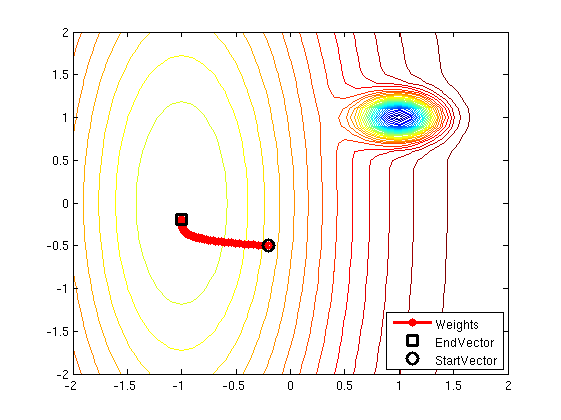
\includegraphics[width=0.8\textwidth]{./figures/211/path_w02_eta01.png}
  \caption{Verlauf von $\vect{w}$}
  \label{fig:path_w02_eta01}
\end{figure}

\begin{figure}[h!]
  \centering
  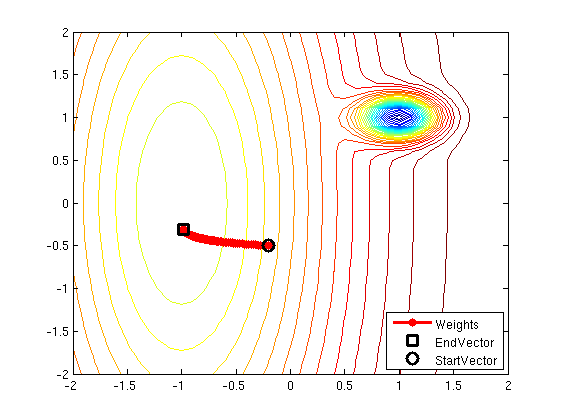
\includegraphics[width=0.8\textwidth]{./figures/211/path_w02_eta005.png}
  \caption{Verlauf von $\vect{w}$}
  \label{fig:path_w02_eta005}
\end{figure}

\begin{figure}[h!]
  \centering
  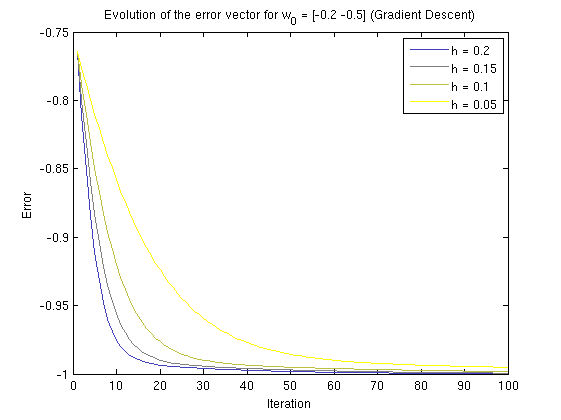
\includegraphics[width=0.8\textwidth]{./figures/211/error_w02.png}
  \caption{Verlauf von $f(\vect{w})$}
  \label{fig:error_w02}
\end{figure}
